\newpage
\appendix
\chapter{Apêndice 1}
\label{apendice1}

\section{Processos de Usabilidade}


	Alguns autores como ~\citeonline{mayhew1999} e ~\citeonline{hix1993} proposeram modelos de processo baseados em ciclo de vidas bem definidos para as atividades de usabilidade. O termo modelo de ciclo de vida é utilizado para representar um modelo que capta um conjunto de atividades e a maneira como elas se relacionam ~\cite{preece2007}. 
	Outro modelo muito utilizado para descrever processos de usabilidade é o proposto pela norma ISO/IEC-13407 (1999).

\subsection{Modelo Estrela}

	Proposto em 1989 por ~\citeauthor{hix1993}, o modelo de ciclo de vida estrela derivou do trabalho empírico de entender como os \emph{designers} lidavam com os problemas de \emph{design} em IHC. Eles observaram dois diferentes modelos de trabalho: analítico e o sintético. O primeiro parte-se da visão do sistema para a visão do usuário, já o segundo da visão do usuário para a do sistema ~\cite{cybis2010}.

	No modelo estrela não há especificação de ordenamento de atividades. Pode-se ir de uma atividade à outra há qualquer momento, desde que passe primeiramente pela avaliação. Sempre que uma atividade for completada deve-se avaliar o seus resultados.

\begin{figure}[h]
    \centering
    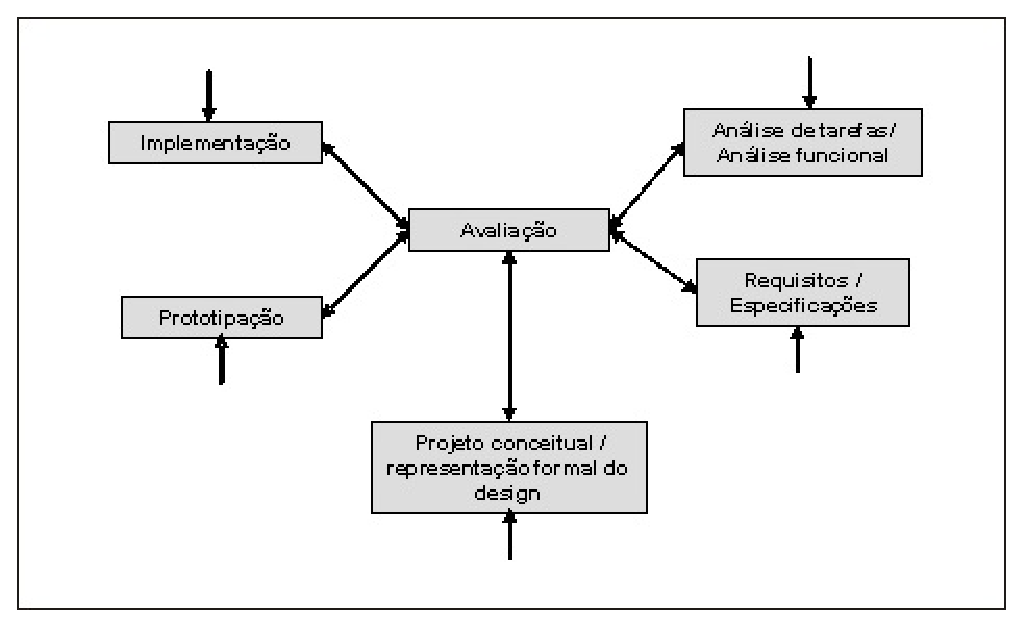
\includegraphics[keepaspectratio=true,scale=0.60]
      {figuras/estrela.eps}
    \caption{Ciclo de Vida Estrela}
    \label{ciclo_estrela}
\end{figure}

\subsection{O ciclo de vida da Engenharia de Usabilidade - Mayhew}

	O ciclo proposto por ~\citeonline{mayhew1999} oferece uma visão holística acerca dessa engenharia e uma descrição detalhada de como podemos realizar os testes de usabilidade % ~\cite{preece2005}.

	A primeira etapa do ciclo é a análise dos requisitos. Mayhew propõe quatro tipos de atividades de análise de requisitos que são detalhadas abaixo:

\begin{itemize}
\item \textbf{Análise do perfil do usuário:} Os projetistas devem conhecer os atributos pessoais e suas habilidades para cada tipo de usuário identificado. 
	
\item \textbf{Análise do contexto da tarefa:} Os projetistas devem conhecer os objetivos e resultados, a estrutura, duração, custos e etc. de cada tarefa a ser realizada.

\item \textbf{Análise das possibilidades e restrições da plataforma:} Verificar quais são as possibilidades e restrições em termos de equipamentos, sistemas operacionais e etc.

\item \textbf{Análise dos princípios gerais para o projeto:} Atividade relacionada à pesquisa e catalogação dos conhecimentos de ergonomia disponível para a concepção da interface no tipo de contexto de uso.

\end{itemize}

	Depois da análise dos requisitos é preciso especificar as metas de usabilidade do futuro sistema. A norma ~\citeonline{iso:9241} orienta como podemos especificar essas metas.

	Na etapa de projetos, testes e implementação, Mayhew propôs que os ciclos devem se repetir de forma a tratar três níveis de aspectos de uma interface: No primeiro nível sendo a interface definida conceitualmente; no segundo nível refere-se as definições em termos de estilo; e no terceiro nível as interações e componentes relacionados com os contextos das tarefas especiais. A última fase é a de instalação do sistema onde depois que o usuário já estiver acostumado com o sistema ele pode dar um \textit{feedback} sobre a usabilidade do produto de forma mais fidedigna por já ser um ``especialista" da ferramenta como cita a autora. 
%
	Uma das técnicas utilizadas para coletar \textit{feedback} são os testes de usabilidade no local do trabalho dos usuários ou utilizando métodos de análise como entrevistas, observações, questionários, grupos de discussões. 

%TODO ISO 13.... (Design centrado no Usuario)

\section{Técnicas e Métodos da Engenharia de Usabilidade}

Esta seção mostra as técnicas e os métodos que são utilizados pela interação humano computador para desenvolver um sistema com usabilidade.
%
De acordo com \\ ~\citeonline{bervian2002metodologia} as técnicas são procedimentos específicos utilizados por uma ciência determinada. O conjunto com várias técnicas constituem os métodos. Algumas técnicas são utilizadas em várias ciências e os métodos se adapta às diversas ciências a medida que há imposição de uso de técnicas especializadas.
%
~\citeonline{cybis2010} divide as técnicas e os métodos da engenharia de usabilidade em três tipos: Concepção, Análise e Avaliação.


\subsection{Métodos e técnicas de concepção}

	Os métodos de concepção são utilizados para implementar as especificações e os requisitos para a interface a usabilidade de um sistema.

\begin{description}

\item[Brainstorming:]

	Bastante utilizado em ambientes ágeis para obter ideias, entrar em consenso sobre problemas ou novas propostas.

\item[Storyboard:]

É uma representação das interações entre os usuários e o sistema em seu ambiente de trabalho. Corresponde ao detalhamento de um cenário de uso especificado para o sistema consistindo em uma sequência de desenhos representando não só os esboços de telas, mas também os elementos do contexto (usuários, equipamentos, móveis, telefones, colegas).

\item[Card Sorting:]

	É uma técnica usada para descobrir como o usuário classifica determinada informação em sua mente. O usuário recebe uma série de cartões embaralhados descrevendo conteúdos e agrupam os cartões que tenham alguma relação. Podem ser distribuídos cartões com nomes de categorias. 
%
O \textit{card sorting} pode ser aberto ou fechado podendo ser aplicado tanto de forma presencial ou remota e aplicados para grupos ou para uma única pessoa. Recomenda-se no mínimo 15 testes e que cada teste tenha 2 pessoas.\footnote{\url{www.uxdesign.blog.br}}
	
\item[Diagramas de Afinidade:]

	São utilizados para organizar uma grande quantidade de itens em grupos lógicos. Diferente do \textit{card sorting}, nesta técnica os projetistas e usuários trabalham juntos para obter consenso sobre a organização dos itens. Essa técnica pode ser usada para analisar os resultados de estudos de campo e analisar as conclusões de uma avaliação de usabilidade.

\item[Protótipos:]

	Os protótipos de papel são úteis para detectar problemas de usabilidade logo no início do proceso de \emph{design}. São usados para esclarecer os requisitos específicos para o projeto da interface do sistema. São rápidos de construir, permitindo rápidas interações de projeto e necessitam de poucos recursos para serem criados. 
	Existem também os protótipos de baixa, média e alta que simulam o sistema com mais fidelidade do que os protótipos em papel. 
\end{description}

%------------------------------------------------------------%%%

\subsection{Métodos e técnicas de análise}

Estes métodos são utilizados para buscar informações sobre o contexto de uso e sobre a usabilidade de um sistema. Podem ser feitas análises do perfil do usuário, o ambiente de uso, as tarefas, possibilidades e restrições do sistema.

As técnicas mencionadas à baixo visam apoiar os projetistas de interface na busca de informações sobre o contexto de uso e sobre a usabilidade de um sistema existente. Essas técnicas são empregadas de forma que se complementem-se umas as outras.

\begin{description}

\item[Observação:]

	Essa técnica caracteriza-se por um pesquisador observando o usuário e tomando notas, enquanto este trabalha em seu contexto usual. É uma técnica útil para obter dados quantitativos (tempo para as tarefas) e qualitativos (práticas e estratégias do usuário). No planejamento é importante definir os objetivos e as maneiras de como será registrada os acontecimentos. Deve-se levar em consideração o fato que muitos usuários por estarem sendo observados podem alterar seu comportamento ao utilizar a ferramenta. É importante que todos estejam cientes dos objetivos do estudo, deixando claro que não é ele que será avaliado e sim conhecer uma situação de uso ~\cite{cybis2010}.

\item[Entrevistas Tradicionais:]

Através de entrevistas podemos obter as opiniões tanto dos usuários atuais como dos futuros usuários dos sistemas. Primeiramente é importante identificar as necessidades das pessoas em acessar uma determinada informação.

\item[Eyetracking:]

É uma técnica que rastreia o movimento dos olhos e da cabeça para registrar a tomada de informações numa interface.

\item[Questionários de Perfil de Uso:]
 
É utilizado para obter informações sobre as características reais dos usuários de um sistema e saber como eles realmente utilizam tais ferramentas. É importante que ao utilizar os questionários de perfil de uso é preciso definir um foco para a sua pesquisa. Deve-se identificar as principais dúvidas da equipe de projeto em relação ao uso do sistema ~\cite{cybis2010}.

Este tipo de questionário pode ser enviado para os \textit{e-mails} dos usuários da ferramenta em análise. É importante definir o tamanho de sua amostra. De acordo com ~\citeonline{cybis2010}, de 20 a 30 por cento é a taxa de retorno dos questionários enviados. As respostas podem ser analisadas utilizando métodos estatísticos.

\label{quest-satisf}
\item[Questionários de Satisfação:]

	A aplicação de questionários é um dos métodos mais utilizados para avaliação da satisfação do usuário. Eles resultam da avaliação subjetiva pelo usuário, o qual é influenciado pelos tipos de questões aplicadas.
	
	Questionários de satisfação são utilizados principalmente quando existem usuários experientes que utilizam o sistema com frequência, podendo ter informações fidedigna sobre aspectos satisfatórios e insatisfatórios no sistema. Também podem ser aplicados por usuários de uma nova versão de um sistema imediatamente após um teste de usabilidade. Essa relação com os testes de usabilidade é interessante por permitir a correlação das medidas de desempenho (tempo, frequência) com as medidas de satisfação do usuário ~\cite{cybis2010}.

	É recomendado que se utilize um questionário padronizado, pois permite a comparação de resultados obtidos por diferentes sistemas. Estes questionários apresentam opções de respostas fechadas, o que permite a produção de dados quantitativos e objetivos ~\cite{cybis2010}.

	Um grande número de questionários foram desenvolvidos pela comunidade científica para a avaliação da usabilidade.  Alguns exemplos de questionários são: QUIS, SUMI,  WAMMI, SUS, ASQ, PSQ, PSSUQ e CSUQ. Os detalhes referentes a cada questionário estão detalhados no apêndice~\ref{apendice1}.

\item[Grupos de Foco:]

É uma reunião informal de usuários que manifestam suas opiniões sobre o determinado assunto, que pode ser tanto uma oportunidade de novas funcionalidades ou algum problema específico.
%
Um moderador deve preparar um roteiro  com uma lista de assuntos a serem tratados. É importante que os participantes sejam de perfis diferentes para que possa ter uma maior diversidade de informações. Costuma-se ter em média de 6 a 12 usuários em uma mesa de reuniões. Os registros das informações podem ser através de vídeos ou blocos de anotações. O objetivo não é ter a obtenção do consenso em torno das ideias, mas sim ter uma boa quantidade de opiniões sobre o assunto a ser tratados ~\cite{cybis2010}.


\item[Diários:]

	É uma técnica útil quando a experiência do usuário é ampla e depende da utilização em muitos lugares. Nessa técnica os usuários carregam consigo um pequeno diário para nele anotar as informações do seu dia-a-dia na utilização do sistema ~\cite{cybis2010}.

\item[Benchmarking de Usabilidade:]

	Definido como método sistemático e contínuo de avaliação de sistemas reconhecidos como representantes das melhores e mais eficazes práticas com a finalidade de comparar desempenhos e identificar oportunidades de melhoria ~\cite{spendolini1994}.

	Esse método parte da definição dos critérios de avaliação e seleção de representantes relevantes para criar uma listagem de características desejáveis para o futuro sistema, como também os aspectos que são desfavoráveis e que devem ser evitados.

\item[Cenários de uso:]

	É uma técnica simples e eficaz para analisar e comunicar uma parte das especificações de requisitos produzidos para a usabilidade e a interface. São utilizados para comunicar os cenários atuais de uma tarefa (problema) e o cenário futuro (solução). Os cenários de solução deve descrever em linguagem natural, como determinados usuários realizarão tarefas específicas com o sistema em um determinado contexto. É preciso decompor os objetivos dos usuários segundo as operações necessárias para alcança-los, identificando as atividades que serão realizadas pelos usuários ~\cite{cybis2010}.

\item[Personas:]

	A técnica de persona descreve o perfil de uma pessoa fictícia envolvida com o produto. Trata-se de inventar um conjunto de pessoas (três ou quatro) que estejam dentro da população de usuários pretendidos e descrevê-las em detalhes.
%
	As informações devem ser qualitativas e coletadas por meio de entrevistas e questionários junto à população alvo do sistema. As personas permitem maior entendimento dos usuários, colocando-os no centro das decisões do projeto. Essa técnica tem objetivos similares aos de cenários, porém ao invés do foco ser na tarefa, deve-se ter foco em uma pessoa que faça parte do público alvo do sistema ~\cite{cybis2010}.

\end{description}

\subsection{Técnicas e Métodos de avaliação}
\label{avaliacao}

\begin{description}

	
\item[Percurso Cognitivo:]

Percurso cognitivo é um método de inspeção de usabilidade que tem como objetivo avaliar a interface considerando a facilidade da interface. A finalidade do percurso cognitivo é fazer com que o \emph{design} de interação seja fácil de aprender por meio da exploração. Os inspetores aplicam uma lista de verificação orientada à tarefa interativa, abordando os processos cognitivos que se estabelecem quando o usuário a realiza pela primeira vez~\cite{cybis2010}.


\item[Teste de Usabilidade:]

É um dos métodos de teste de experiência do usuário (UX) mais frequentemente utilizado e conhecido entre aqueles que não são projetistas da UX. Realizar testes com usuários é o núcleo do \emph{Design} Centrado no Usuário, pois é através destes que podemos saber se as reais expectativas dos usuários são atendidas ~\cite{santos2012}.
%
O teste consiste em avaliar o desempenho dos usuários na execução de tarefas cuidadosamente preparadas, tarefas estas dentro do escopo do sistema. Esse desempenho pode ser avaliado no quesito, número de erros e tempo de execução da tarefa, questionários e entrevistas também podem ser utilizados ~\cite{preece2007}. Na próxima seção será detalhado os passos comuns que devem ser seguidos para a execução dos testes de usabilidade.

\end{description}

	As técnicas descritas nessa seção podem ser associadas com várias outras técnicas e para a escolha de cada técnica é importante examinar as possibilidades dos recursos necessários e os disponíveis e as expectativas de resultados da avaliação da usabilidade. Cada técnica apresentam qualidades diferentes em relação à quantidade de problemas que as identificam, sistematização dos resultados, à facilidade da aplicação. 
%

\section{Testes de Usabilidade}
\label{testes_u}
{	Existem vários tipos de testes de usabilidade, mas sabe-se que todos eles têm algo em comum, que é observar as pessoas utilizando algo.
}

\begin{itemize}

	\item \textbf{Escolher abordagem}

	As abordagens de pesquisa podem ser de dois tipos: quantitativa ou qualitativas. 
	%
	As pesquisas quantitativas são focadas nos dados numéricos e é voltada para fornecer alta confiança e resultados repetidos dentro de seus grupos de usuários. É preciso ter o envolvimento de um número maior de participantes para contar as variações que você encontrará de indivíduo para indivíduo ~\cite{unger2009}.
	%
	As pesquisas qualitativas não são focadas em níveis de segurança e da possibilidade de repetição, mas sim ganhar contexto e percepção considerando o comportamento do usuário. Ela depende da interpretação do projetista sobre as descobertas, a intuição e o senso comum ~\cite{unger2009}.

	Os testes quantitativos são como experimentos científicos que precisam ser rigorosos ou os resultados não serão confiáveis. Deve-se definir um protocolo de teste e segui-lo consistentemente para todos os participantes ~\cite{krug2010}.
	%
	Nos testes qualitativos você tenta minimizar a quantidade de interação com o participante para evitar a influência nos resultados ~\cite{krug2010}.

	Para os testes de usabilidade é possível utilizar qualquer uma das abordagens, mas a qualitativa é a mais acessível para aqueles que não tiveram um treinamento em métodos científicos mais formais e oferece uma rica fonte de dados ~\cite{unger2009}.


	\item \textbf{Planejar a pesquisa}

	Algumas questões devem ser respondidas ao criar o teste de usabilidade: Estas questões te ajudam a oferecer foco e escopo. Abaixo algumas perguntas que devem ser respondidas no planejamento de sua pesquisa:

	\begin{itemize}
		\item Defina seu objetivo: Por que você está testando? 
	\item Defina Usuários: Quem você está testando? 
	\item Defina o método para representar sua aplicação: O que você está testando?
	\item Quais informações você está reunindo? 
	\end{itemize}
	
	

Nas pesquisas qualitativas geralmente queremos compreender as questões que os usuários podem encontrar, os níveis de frustrações que eles podem experimentar e a gravidade de um problema em particular. Para os testes qualitativos devem se pensar em medidas que serão possíveis de ser respondidas com cinco usuários ~\cite{unger2009}. 

	\begin{itemize}
		\item Taxa de Sucesso: O grau em que o usuário foi capaz de completar a tarefa.
		%Pode-se detalhar com mais informações sobre o que seria a taxa de sucesso, e o que é considerado o sucesso.
		\item Satisfação do usuário
	\end{itemize}
	

\item \textbf{Usuários}

Existem algumas diretrizes que podem ser adotadas para a definição da quantidade de usuários. ~\citeonline{nielsen1994} definiu algumas dessas diretrizes:

\begin{itemize}
\item No teste quantitativo planeje uma quantidade maior de participantes. Em média 20 por rodada de pesquisa.
\item No teste qualitativo é suficiente ter entre 5 e 8 participantes.
\end{itemize}

	 ~\citeonline{krug2010} defende a ideia de que três usuários são ideais para realização de testes de usabilidade para quem está realizando o teste por conta própria. Ele afirma que é mais fácil encontrar três participantes do que uma quantidade maior e que é bem provável que eles já encontrem muitos dos problemas significativos relacionados as tarefas que você está testando.

	Em equipes ágeis, o teste com o usuário é realizado com o cliente do projeto e envolve o especialista em usabilidade como mediador do teste ~\cite{santos2012}.

\item \textbf{Recrutamento e logística}

Depois de ter feito o plano de pesquisa e definido os tipos de usuários que podem ser inseridos na pesquisa é hora de recrutar os participantes.
Para o recrutamento de participantes é interessante gerar uma lista com os potenciais participantes do teste. Essa lista pode vir de usuários registrados do site da empresa relacionada; informações de contatos do cliente; \textit{e-mails} para conhecidos que tenha relação com o assunto do teste; requisições em pequenas pesquisas que pré-qualificam os participantes, e etc.~\cite{unger2009}.

Você pode realizar uma filtragem com os participantes potenciais antes de seleciona-los. As perguntas do questionário de filtragem devem ser voltadas para:

	\begin{itemize}
	\item Garantir que o participante seja um usuário das funções em que você está testando.
	\item Determinar se ele se encaixa em um dos seus grupos de usuários.
	\item Ajudar a ter uma boa mistura de participantes.
	\end{itemize}	

O questionário de perfil de usuário pode ser utilizado para realizar essa filtragem de participantes.


\item \textbf{Criação de guias de discussão}

Para a execução do teste de usabilidade é preciso que as instruções estejam claras aos participantes, contendo todas as informações específicas que ele precisará para completar as tarefas com sucesso.

Os seus materiais de teste deve incluir:

		\begin{itemize}
		\item Formulário de consentimento para gravação de vídeo
		\item Guia de discussão para o participante, com tarefas detalhadas e perguntas sobre a satisfação do usuário.
		\item Questionários
		\end{itemize}
		
\end{itemize}


\section{Questionário de Satisfação}

	Levantamos informações sobre alguns questionários de satisfação de uso existentes na literatura e foi feito uma comparação entre cada um deles.

\subsection{QUIS - Questionnaire for User Interaction Satisfaction}

	O QUIS mede a satisfação do usuário quanto â usabilidade do produto de maneira padronizada, segura e válida, a fim de obter informações precisas em relação à reação dos usuários a novos produtos (QUIS, 2009);

	A versão atual é a QUIS 7.0 (Norman e Shneiderman, 2010), contém um questionário onde possui a avaliação da satisfação geral e avaliações de fatores específicos de interfaces organizadas hierarquicamente: tela, terminologia e retroalimentação do sistema, aprendizado, capacidades do sistema, manuais técnicos, tutoriais online, multimídia, teleconferência e instalação de software. Pode ser configurado de acordo com a necessidade e interesse do usuário. 

	É um questionário proprietário, é sugerido o uso de planilhas eletrônicas e softwares estatísticos até que se implementem recursos de análise no servidor web dos proprietários.

\subsection{SUS – System Usability Scale}

	O SUS é uma escala de usabilidade do tipo Likert que possui uma visão global e subjetiva em suas avaliações de usabilidade. Ele apresenta ao entrevistado uma lista de perguntas que devem ser respondidas em uma escala de satisfação (indica o grau de concordância ou discordância do usuário) \cite{brooke1996sus}.

	O autor se baseou na afirmação de que no contexto industrial, as avaliações completas não são práticas e requerem muito esforço e custo. O SUS foi criado pela necessidade de se ter uma avaliação de usabilidade simples e rápida. Os métodos de avaliação foram simplificados e o número de questões reduzidas, pois uma quantidade grande de questões desanima os usuários que possivelmente não preencheria todas as questões, resultando assim problemas na captura de reações subjetivas do usuário. Foi então proposto um questionário com 10 questões que utiliza a escala Likert de cinco ou sete pontos. Este questionário abrange vários aspectos da usabilidade, tais como: necessidade de suporte, treinamento e complexidade. ~\cite{preece2007}

\subsection{SUMI – Usability Measurement Inventory}

	O SUMI proposto por ~\citeonline{kirakowski1988measuring} é um questionário para medição da qualidade de um software do ponto de vista do usuário, é um método consistente usado para avaliar a qualidade de uso de um produto de software ou protótipo, e pode ajudar na descoberta de falhas de usabilidade. É mencionado na norma ISO 9241 como um método reconhecido para testar a satisfação do usuário. O SUMI é um questionário comercial. 

	Inicialmente continha 150 itens onde o participante escolhia se (concordo fortemente, concordo, não sei, discordo ou discordo totalmente). Atualmente são 50 itens divididos em 5 grupos de 10 itens. Os grupos de itens são: eficiência, afeto, eficácia, controle e aprendizado. Os entrevistados preenchem o questionário no seu local de trabalho e devem decidir entre as opções: concordo, não sei ou discordo totalmente.

\subsection{ASQ – The After-Scenario Questionnaire}

O ASQ é um questionário de três itens que são utilizados para avaliar a satisfação do usuário após a conclusão de cada cenário/tarefa. São realizadas umas séries de tarefas que estão de acordo com a realidade do usuário.Este questionário aborda questões como: facilidade de conclusão da tarefa, tempo para completar uma tarefa e adequação das informações de suporte.São questões do tipo Likert, aplicando uma escala de 1 a 7, onde 1 representa “ Concordo totalmente ” e 7 para “ Discordo totalmente ”. ~\cite{lewis1995ibm}

O participante gasta em média 1 hora pra realizar cada cenário, no fim de cada cenário é preenchido o questionário ASQ. Após completar todos os cenários, no fim de 1 dia de trabalho (8 horas), os participantes preenchem o questionário PSSUQ para avaliação geral do sistema.O ASQ foi aplicado na IBM por diferentes tipos de usuários, cada grupo possuía um tempo de experiência com sistemas de computador, o que permitiu a análise psicométrica do questionário.

\begin{figure}[!h]
    \centering
    \includegraphics[keepaspectratio=true,scale=0.60]
      {figuras/asq.eps}
    \label{ASQ - The After-Scenario Questionnaire }
	\caption{ASQ - The After-Scenario Questionnaire}
\end{figure}

\subsection{PSQ – The Printer-Scenario Questionnaire}

O PSQ  é uma versão inicial do ASQ, mas difere no formato e numero de itens.  São escalas de 5 pontos com os termos “ Aceitável ” com nota 1 e “ Precisa de muita Melhoria ” com nota 5, e não marcado “ Para Avaliar ” ~\cite{lewis1995ibm}.

\subsection{PSSUQ – The Post-Study System Questionnaire}

	O PSSUQ fornece uma avaliação global do sistema utilizado. Esse questionário possui 19 itens para avaliação da satisfação do usuário com a usabilidade do sistema. É gasto em média 10 minutos para completar o questionário, mas só é preciso completar uma vez o questionário no fim do estudo de usabilidade. ~\cite{lewis1995ibm} 

	Este questionário ajuda a entender quais aspectos do sistema o usuário está mais preocupado. Ele avalia as características como facilidade de uso e de aprendizado, simplicidade, eficácia, informação e a interface com o usuário.

	Existem 4 tipos de pontuações para as respostas aos itens do PSSUQ: Escore da satisfação geral (OVERALL), a utilidade do sistema(SYSUSE), a qualidade da  informação (INFOQUAL) e a qualidade da interface (INTERQUAL). 

A escala Global está relacionada com a soma das classificações ASQ que os participantes deram após completar cada cenário. 

%fonte lewis2002psychometric

\begin{figure}[!h]
    \centering
    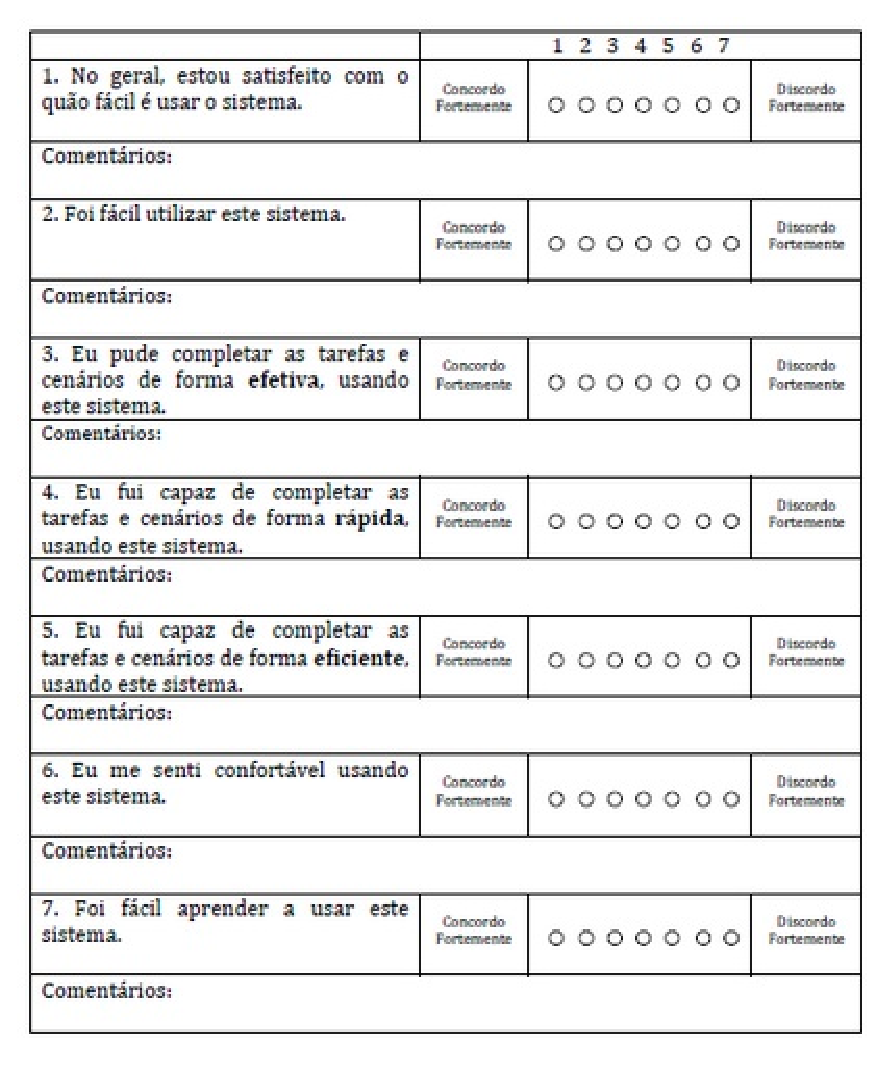
\includegraphics[keepaspectratio=true,scale=0.60]
      {figuras/pssuq01.eps}
    \label{pssuq}
	\caption{PSSUQ – The Post-Study System Questionnaire}
\end{figure}

\newpage

\begin{figure}[!h]
    \centering
    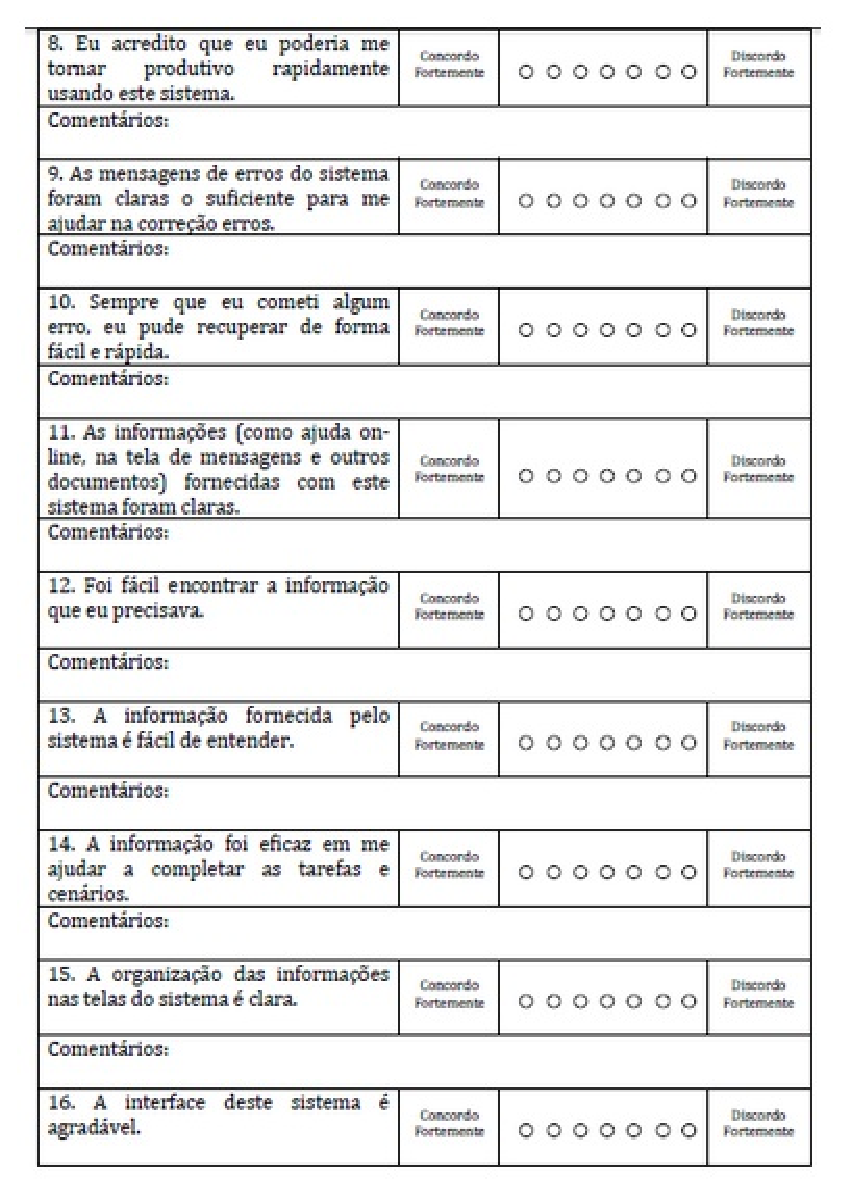
\includegraphics[keepaspectratio=true,scale=0.60]
      {figuras/pssuq02.eps}
    \label{pssuq}
\end{figure}

\begin{figure}[!h]
    \centering
    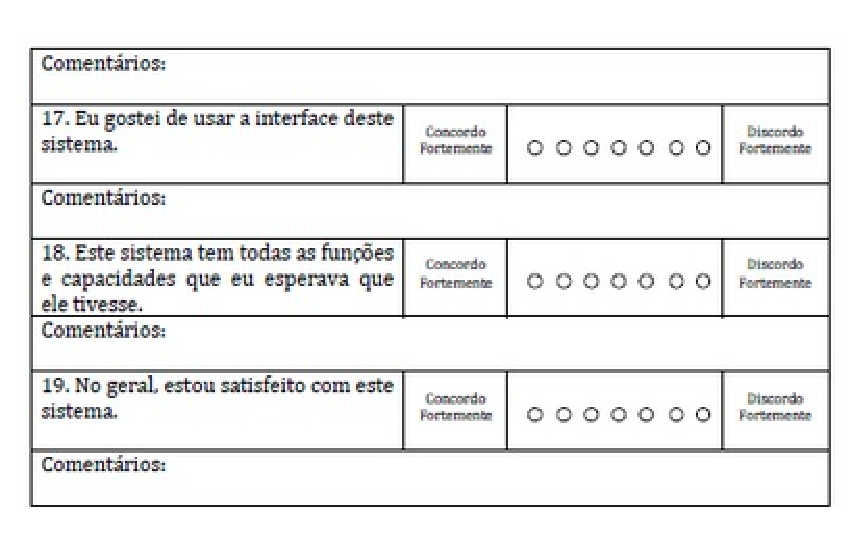
\includegraphics[keepaspectratio=true,scale=0.60]
      {figuras/pssuq03.eps}
    \label{pssuq}
	\caption{PSSUQ: The Post-Study System Questionnaire - Questões de 8 à 19}
\end{figure}

\subsection{CSUQ - Computer System Usability Questionnaire}

	Este questionário é parecido com o PSSUQ, mas a sua redação e diferente. Enquanto no PSSUQ afirma que “ Eu poderia efetivamente realizar as tarefas e cenários usando este sistema ” o CSUQ escreve: “ Eu posso terminar meu trabalho de forma eficaz usando esse sistema?”. Na IBM, este questionário foi aplicado através de e-mail, enviado para funcionários de diferentes locais, o que houve uma maior quantidade de participantes, do que feito com grupos reduzidos presencialmente. ~\cite{lewis1995ibm} 
	O CSUQ é utilizado quando o estudo de usabilidade é em um ambiente fora do laboratório. A confiabilidade relatada foi de 0,93.



\subsection{Comparativo dos questionários}

	Os questionários ASQ e PSQ são utilizados após a realização de um cenário. Contém os mesmos itens, mas possuem escalas diferentes. O ASQ possui uma maior confiabilidade em relação ao PSQ. 

	PSSUQ e CSUQ são ambos os questionários de satisfação global. O PSSUQ utiliza itens adequados para uma situação de teste de usabilidade, já o CSUQ são apropriados para uma situação de teste de campo. Os questionários possuem propriedades psicométricas aceitáveis de usabilidade e podem ser usados com confiança como medidas padronizadas de satisfação. É interessante utilizar o PSSUQ junto com o ASQ.

	O ideal é que o questionário seja mais genérico possível. Cada questionário possui um nível de confiança.

\begin{table}[h]
\begin{tabular}{|l|l|l|l|p{3cm}|l|l|}
\hline
\textbf{Nome} & \textbf{Criador} & \textbf{Questões} & \textbf{Licença} & \begin{tabular}[c]{@{}l@{}}\textbf{Interface  Avaliada}\end{tabular}  & \textbf{Confiab.} & \textbf{Escala} \\ \hline
ASQ & IBM & 3 & Aberto & Qualquer & 0,93 & \begin{tabular}[c]{@{}l@{}}Discordo \\ Fortemente /\\ Concordo \\ Fortemente\end{tabular} \\ \hline
\begin{tabular}[c]{@{}l@{}}CSUQ\end{tabular}    & IBM              & 19       & Aberto          & \begin{tabular}[c]{@{}l@{}}Baseado em\\ computador \end{tabular} & 0,95           & \begin{tabular}[c]{@{}l@{}}Discordo \\Fortemente /\\ Concordo \\ Fortemente\end{tabular} \\ \hline
\begin{tabular}[c]{@{}l@{}}PSSUQ\end{tabular} & IBM              & 19       & Aberto          & \begin{tabular}[c]{@{}l@{}}Baseado em\\ computador \end{tabular} & 0,96           & \begin{tabular}[c]{@{}l@{}}Discordo \\ Fortemente /\\ Concordo\\ Fortemente\end{tabular} \\ \hline
\begin{tabular}[c]{@{}l@{}}SUMI\end{tabular}   & HERG             & 27       & Proprietário    & Software              & 0,89           & \begin{tabular}[c]{@{}l@{}}Discordo \\Fortemente /\\ Concordo\\ Fortemente\end{tabular} \\ \hline
SUS                                                                 & DEC              & 10       & Aberto          & Qualquer              & 0,85           & \begin{tabular}[c]{@{}l@{}}Discordo \\Fortemente / \\Concordo \\Fortemente    \end{tabular}                                         \\ \hline
QUIS                                                                                         & UMD              & 50       & Proprietário    &       -         &       -         & 0 a 9                                                                               \\ \hline
\end{tabular}
\caption {Comparativo dos questionários}
\end{table}


\section{\textit{Checklist} de Usabilidade}
\label{checklist}

	Este checklist contém questões especializada em aspectos ou critérios que determinam a ergonomia de uma interface homem-computador.

	\begin{figure}[!h]
    	\centering
    	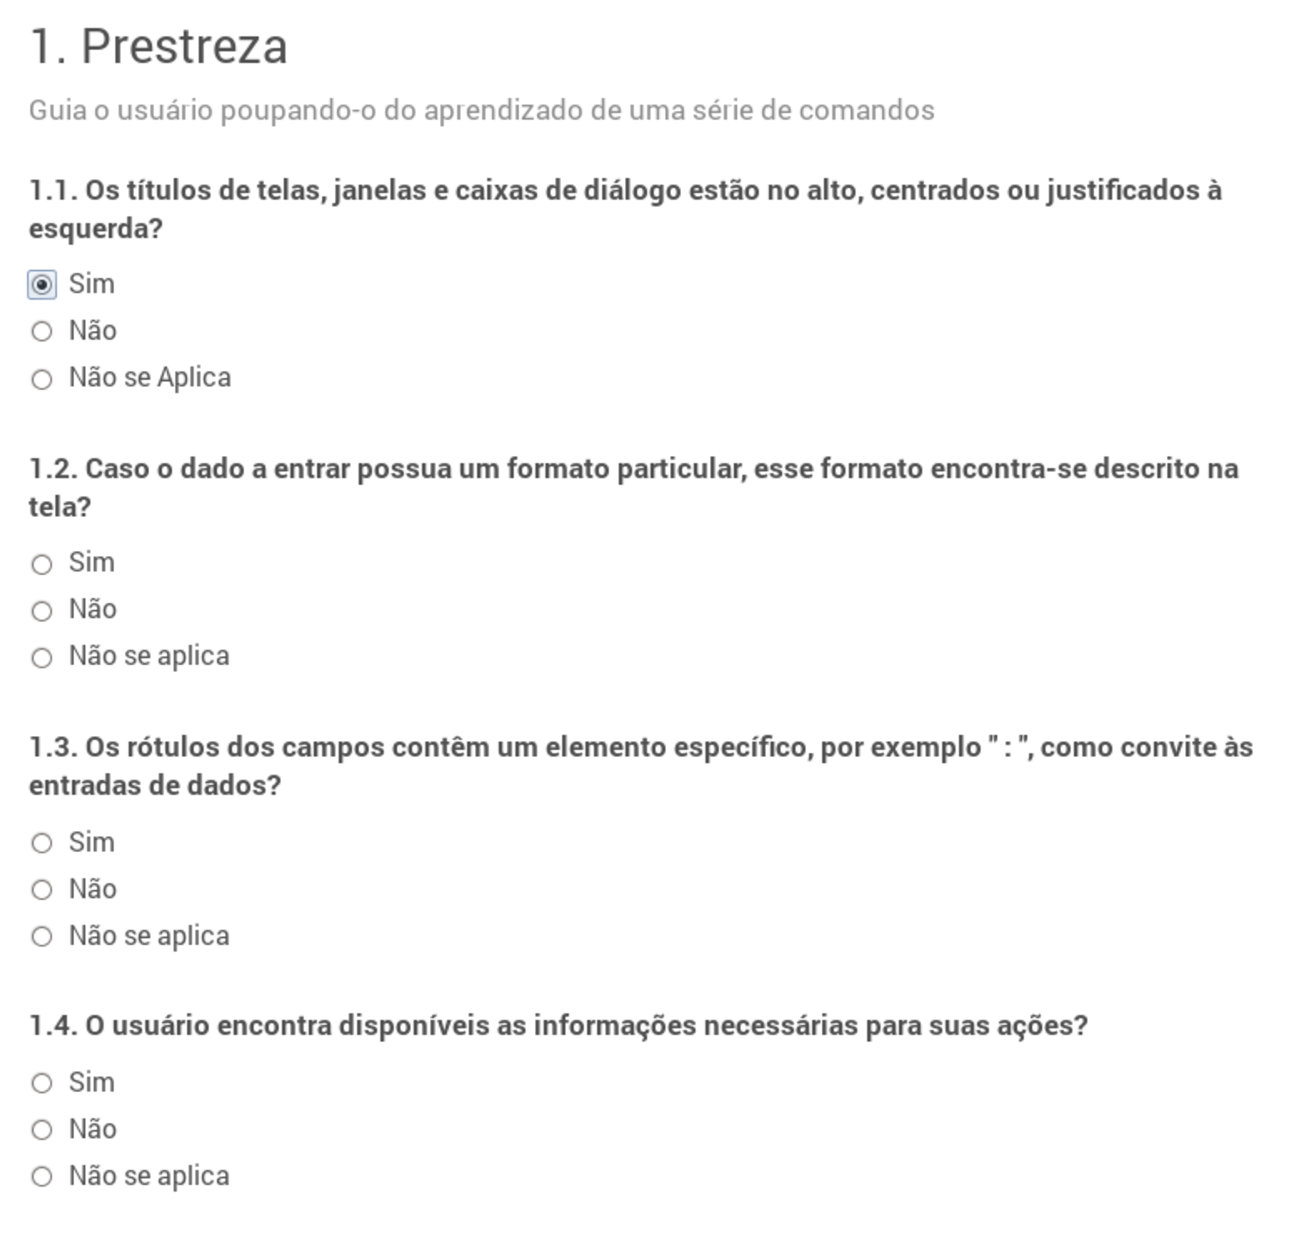
\includegraphics[keepaspectratio=true,scale=0.55]
      		{figuras/check01.eps}
    	\label{check01}
		\caption{Checklist de usabilidade- Questões da seção 01}
	\end{figure}
  
	\begin{figure}[!h]
    	\centering
    	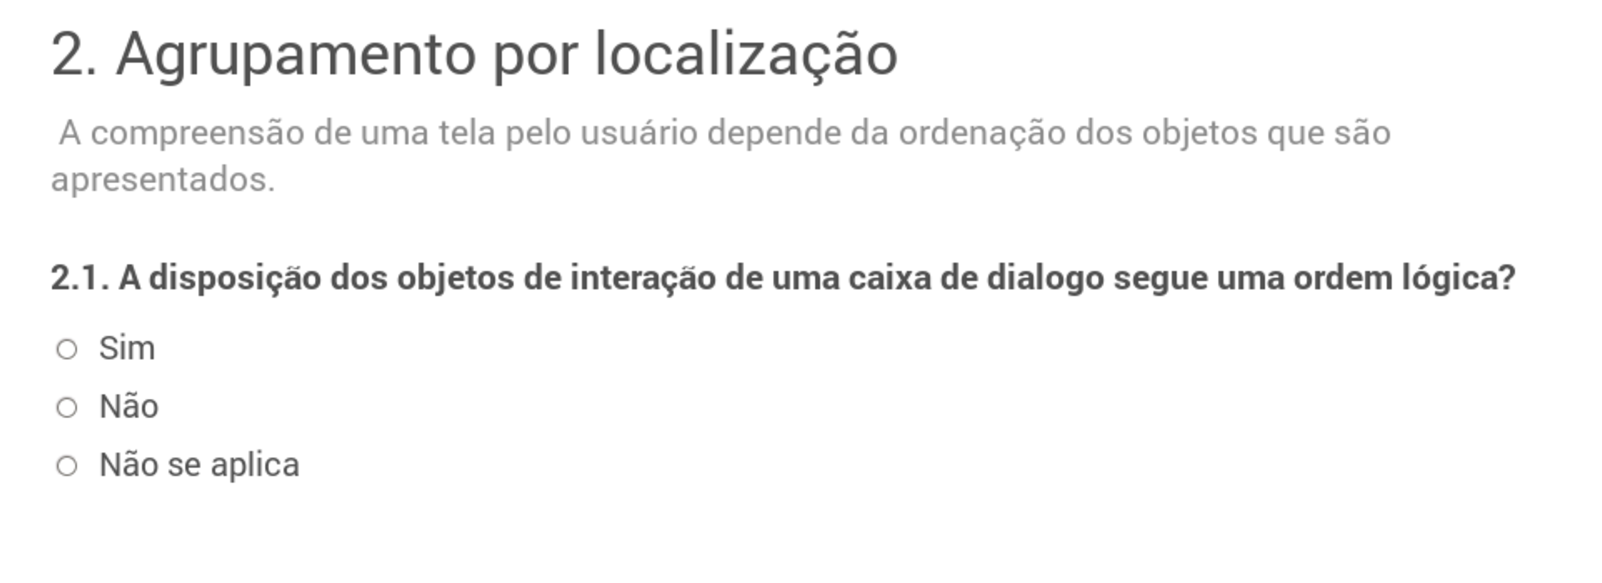
\includegraphics[keepaspectratio=true,scale=0.45]
      		{figuras/check02.eps}
    	\label{check02}
		\caption{Checklist de usabilidade- Questões da seção 02}
	\end{figure}

	\begin{figure}[!h]
    	\centering
    	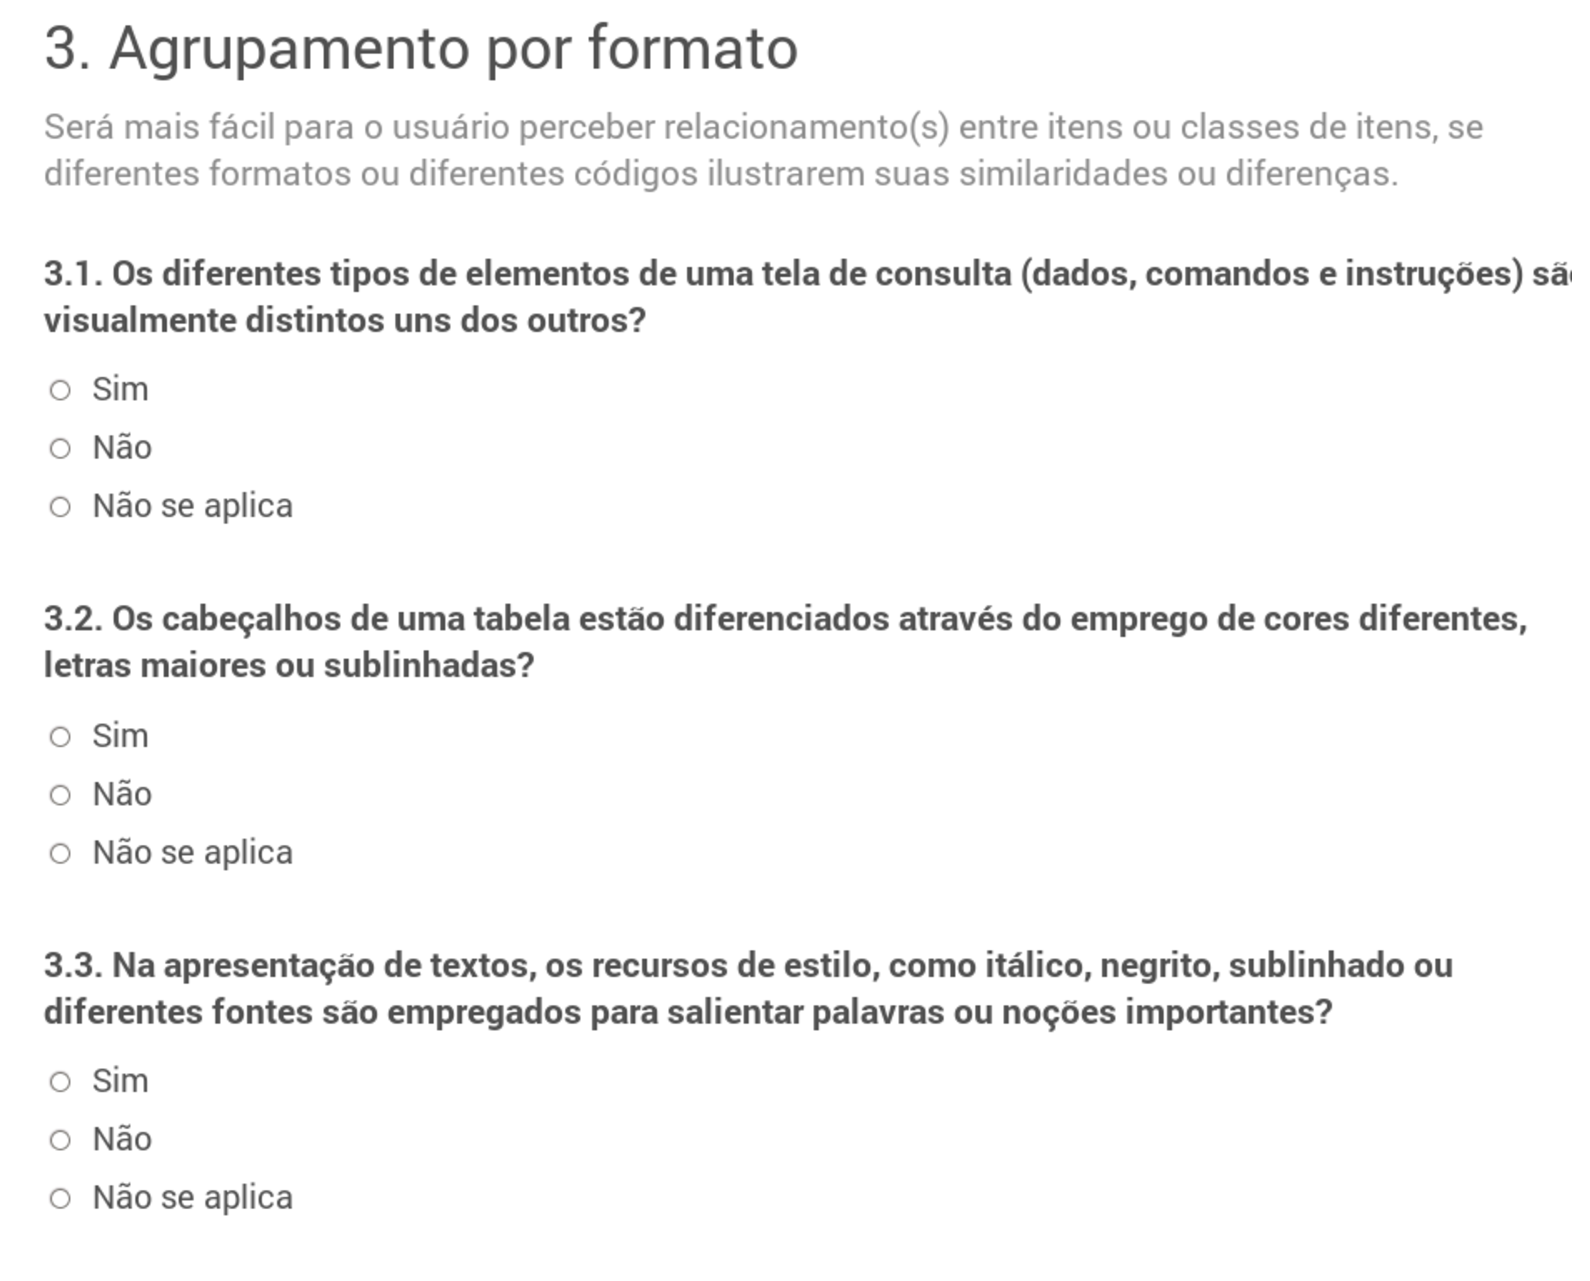
\includegraphics[keepaspectratio=true,scale=0.45]
      		{figuras/check03.eps}
    	\label{check03}
		\caption{Checklist de usabilidade- Questões da seção 03}
	\end{figure}

	\begin{figure}[!h]
    	\centering
    	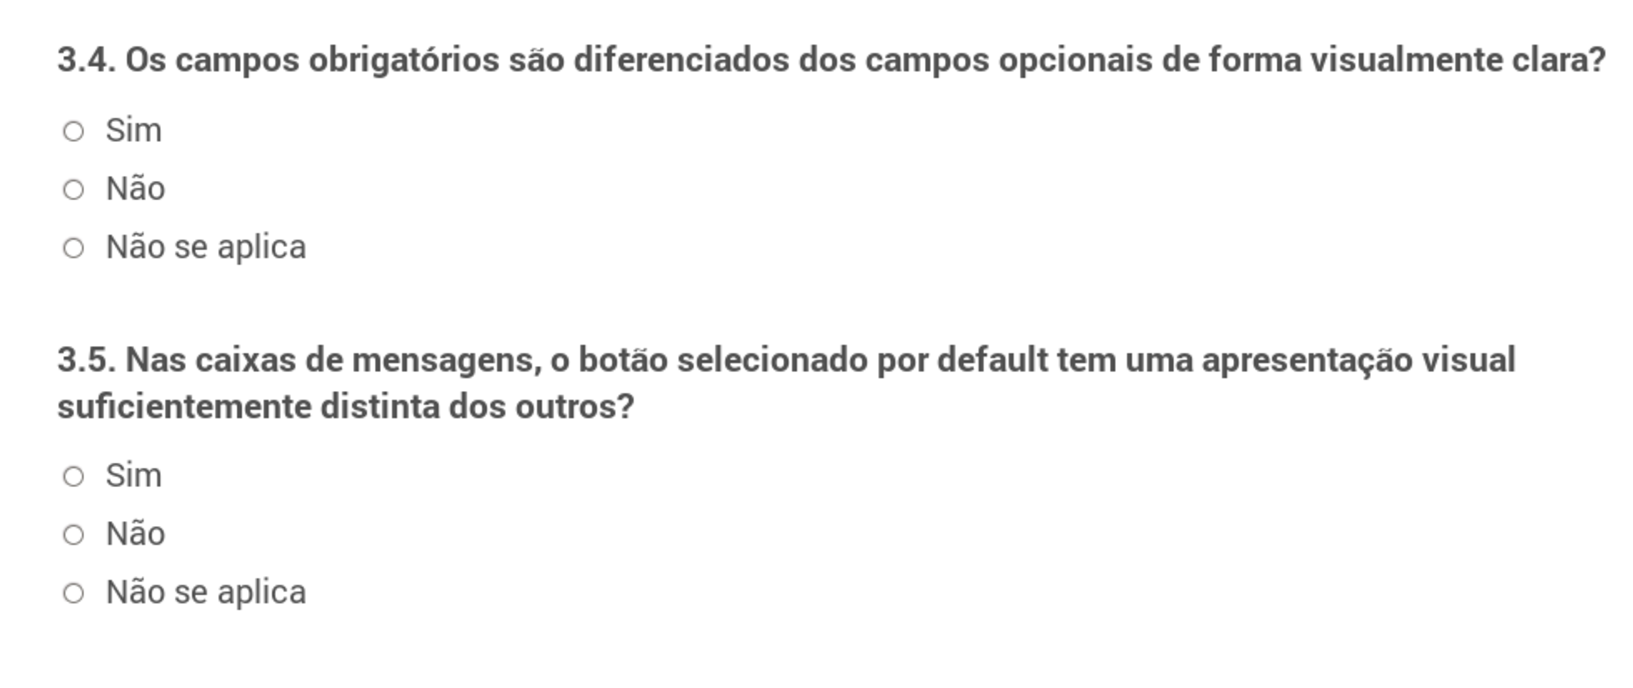
\includegraphics[keepaspectratio=true,scale=0.45]
      		{figuras/check03_2.eps}
    	\label{check03_2}
		\caption{Checklist de usabilidade- Questões da seção 03}
	\end{figure}

	\begin{figure}[!h]
    	\centering
    	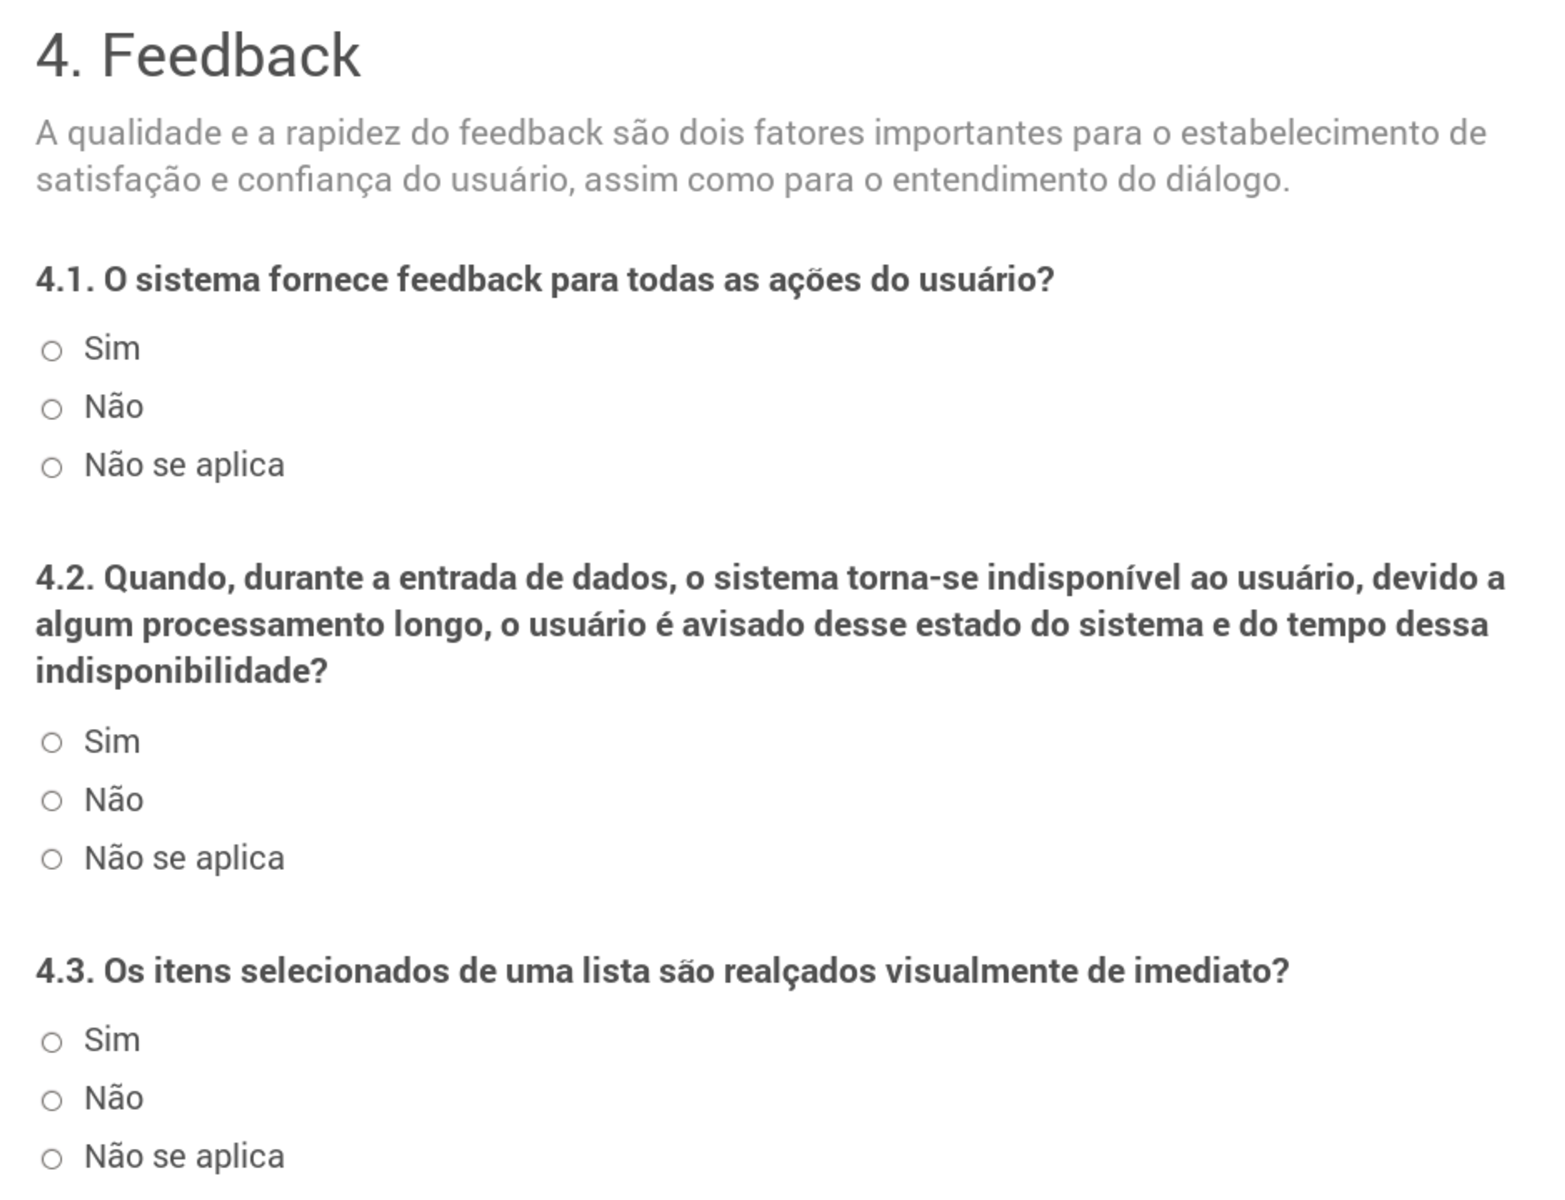
\includegraphics[keepaspectratio=true,scale=0.45]
      		{figuras/check04.eps}
    	\label{check04}
		\caption{Checklist de usabilidade- Questões da seção 04}
	\end{figure}

	\begin{figure}[!h]
    	\centering
    	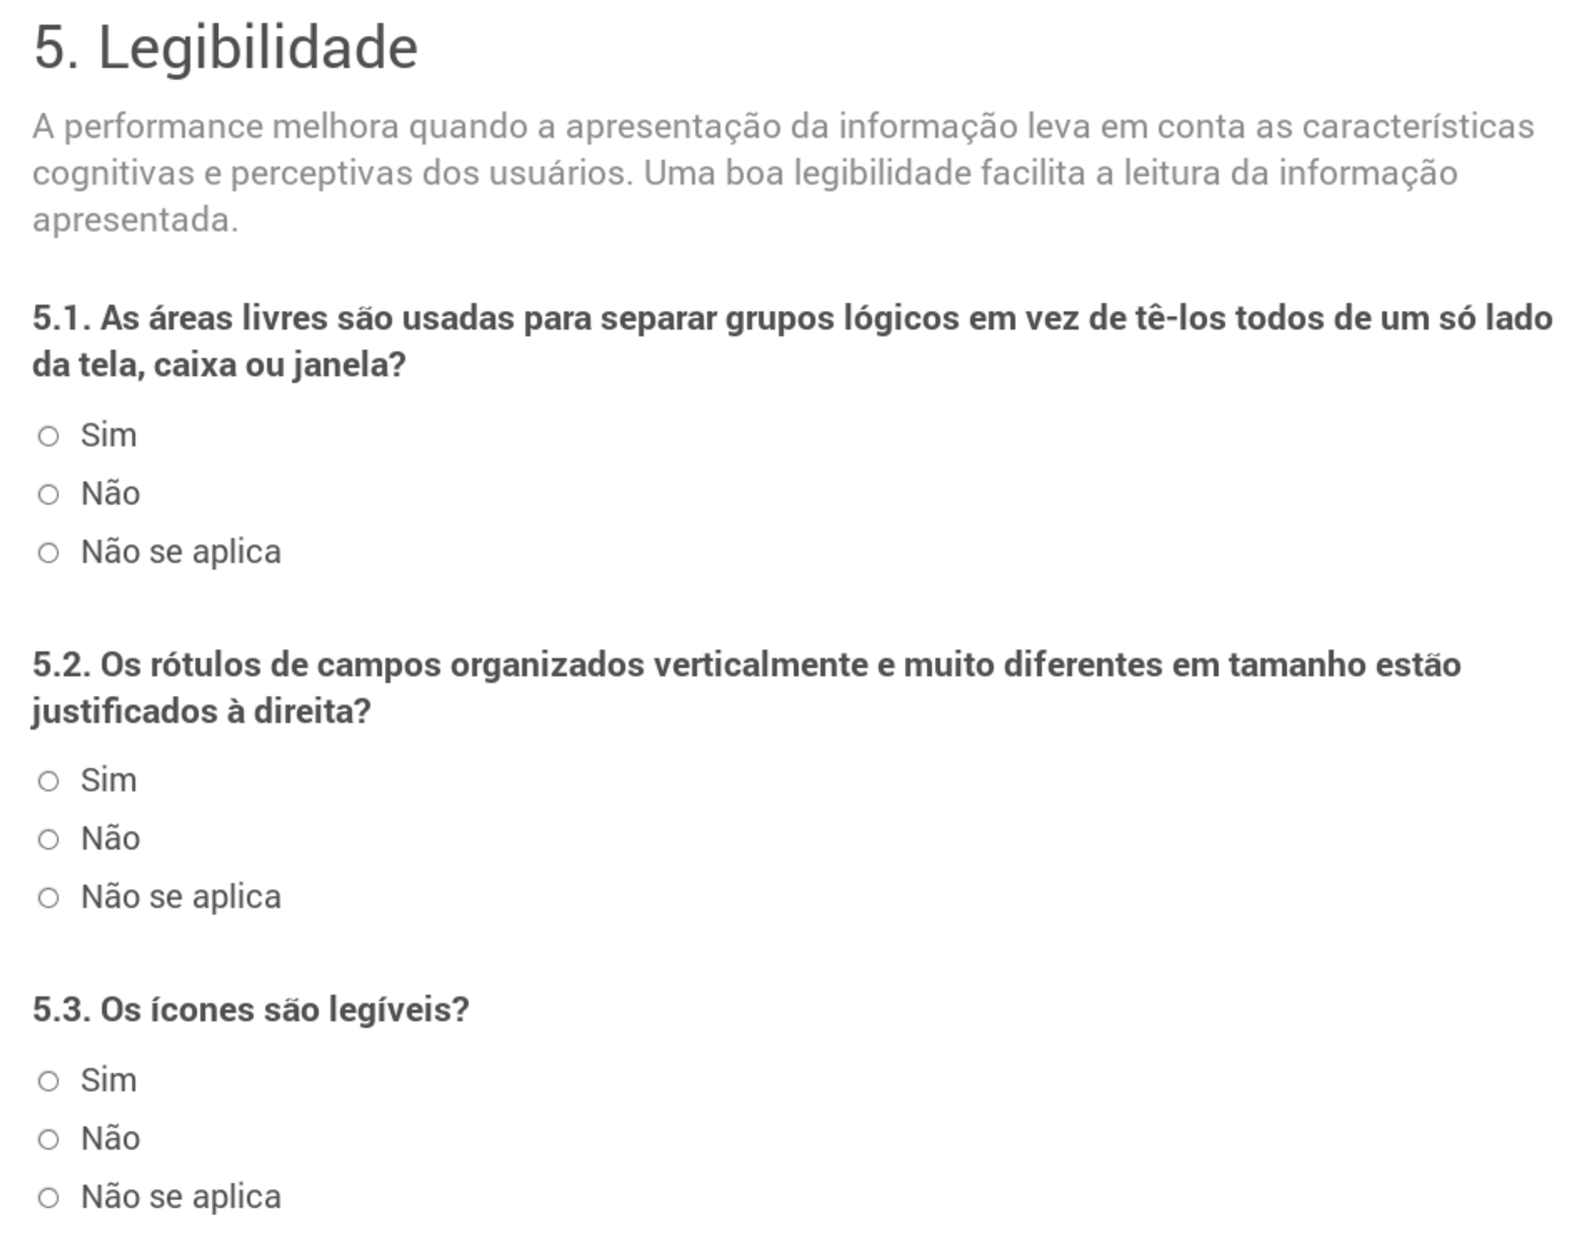
\includegraphics[keepaspectratio=true,scale=0.45]
      		{figuras/check05.eps}
    	\label{check04}
		\caption{Checklist de usabilidade- Questões da seção 05}
	\end{figure}

	\begin{figure}[!h]
    	\centering
    	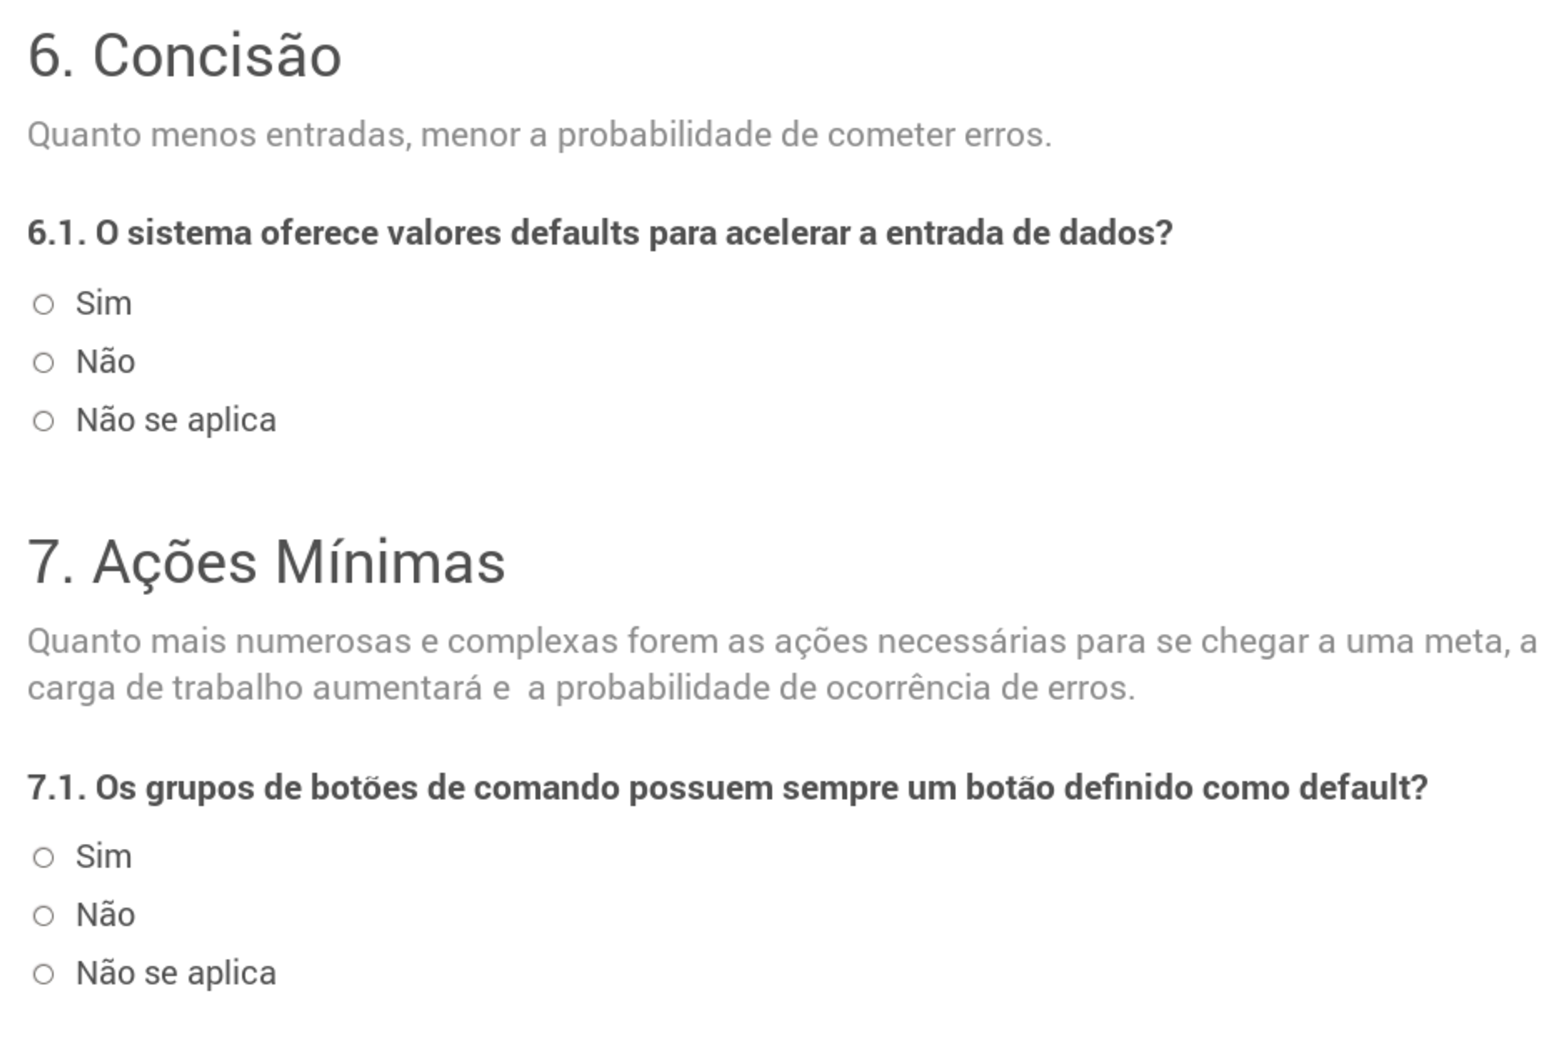
\includegraphics[keepaspectratio=true,scale=0.45]
      		{figuras/check06.eps}
    	\label{check04}
		\caption{Checklist de usabilidade- Questões das seções 06 e 07}
	\end{figure}


	\begin{figure}[!h]
    	\centering
    	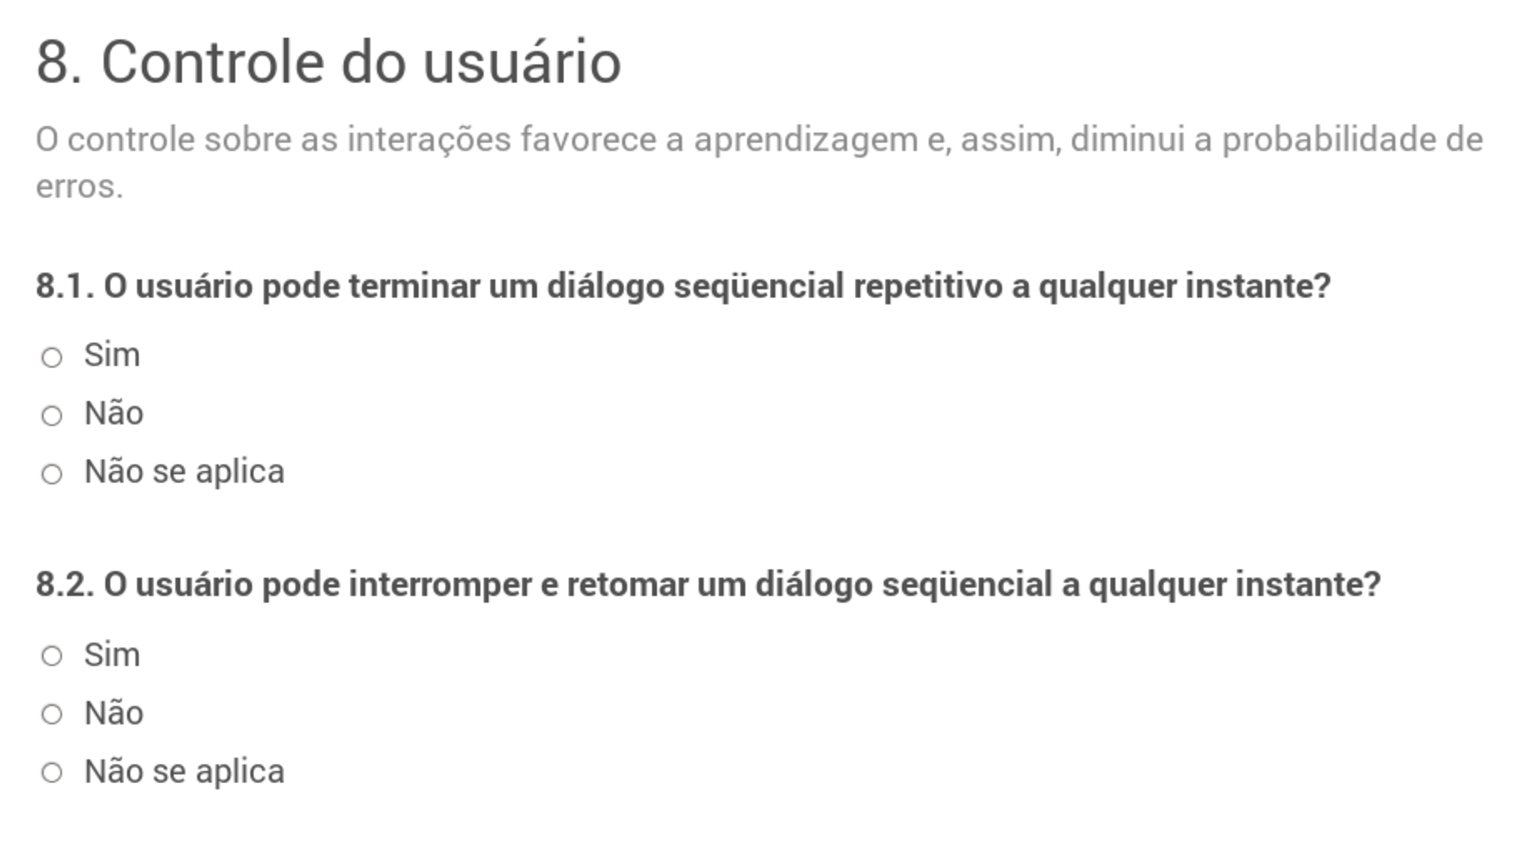
\includegraphics[keepaspectratio=true,scale=0.45]
      		{figuras/check08.eps}
    	\label{check04}
		\caption{Checklist de usabilidade- Questões da seção 08}
	\end{figure}

	\begin{figure}[!h]
    	\centering
    	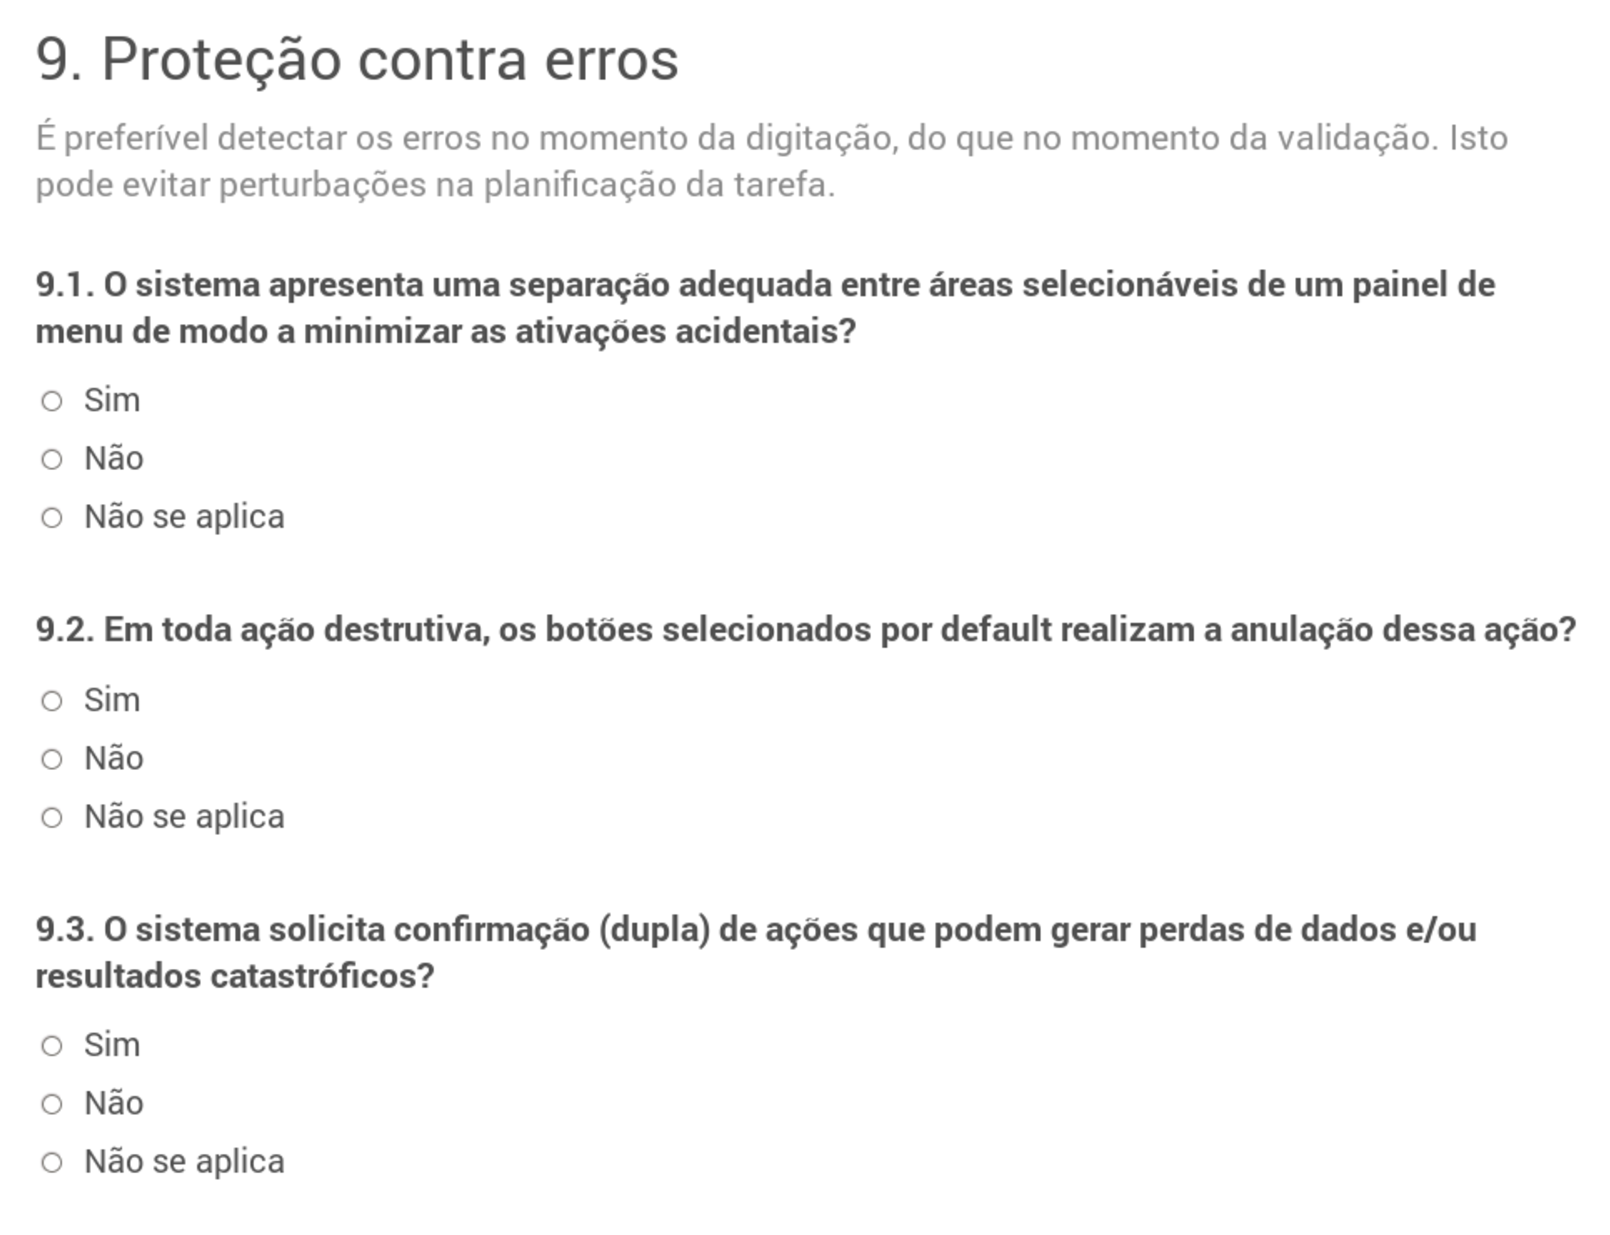
\includegraphics[keepaspectratio=true,scale=0.45]
      		{figuras/check09.eps}
    	\label{check04}
		\caption{Checklist de usabilidade- Questões da seção 09}
	\end{figure}

	\begin{figure}[!h]
    	\centering
    	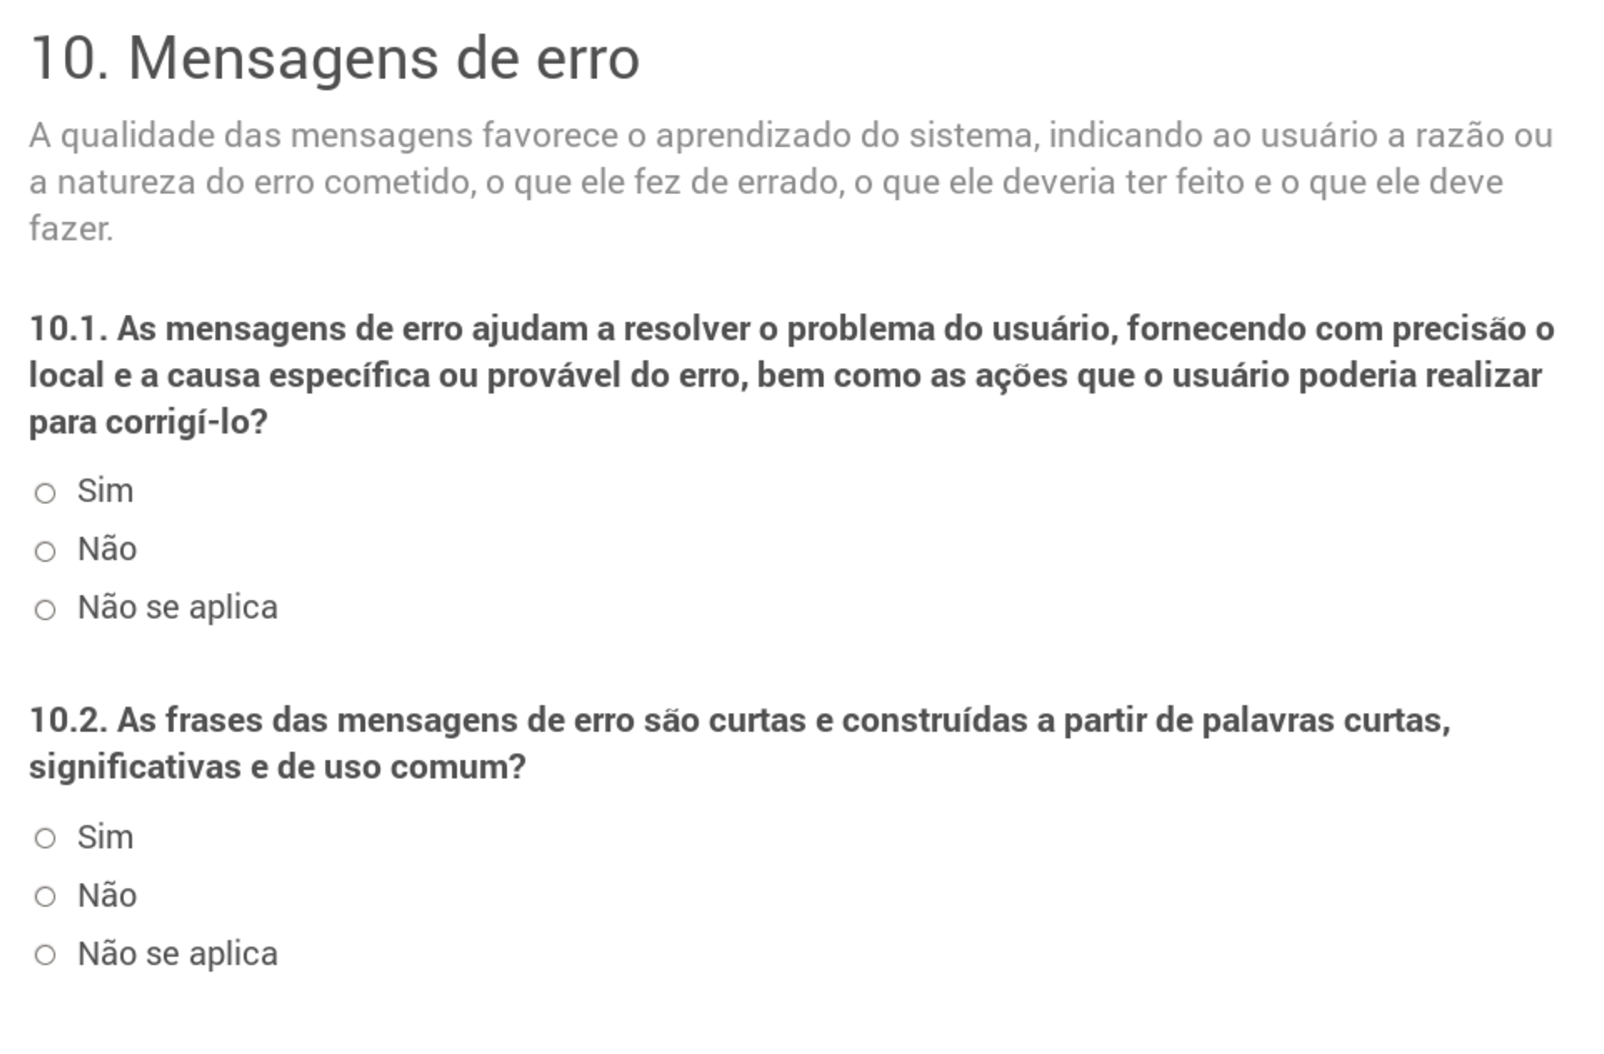
\includegraphics[keepaspectratio=true,scale=0.45]
      		{figuras/check10.eps}
    	\label{check04}
		\caption{Checklist de usabilidade- Questões da seção 10}
	\end{figure}

	\begin{figure}[!h]
    	\centering
    	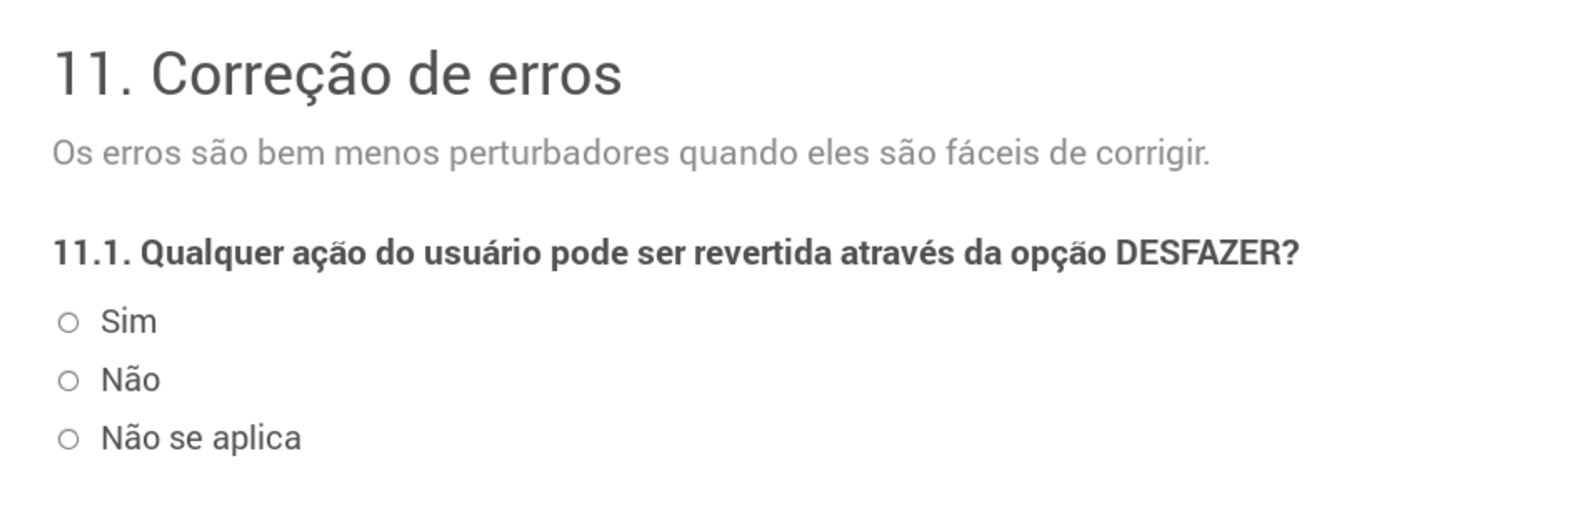
\includegraphics[keepaspectratio=true,scale=0.45]
      		{figuras/check11.eps}
    	\label{check04}
		\caption{Checklist de usabilidade- Questões da seção 11}
	\end{figure}

	\begin{figure}[!h]
    	\centering
    	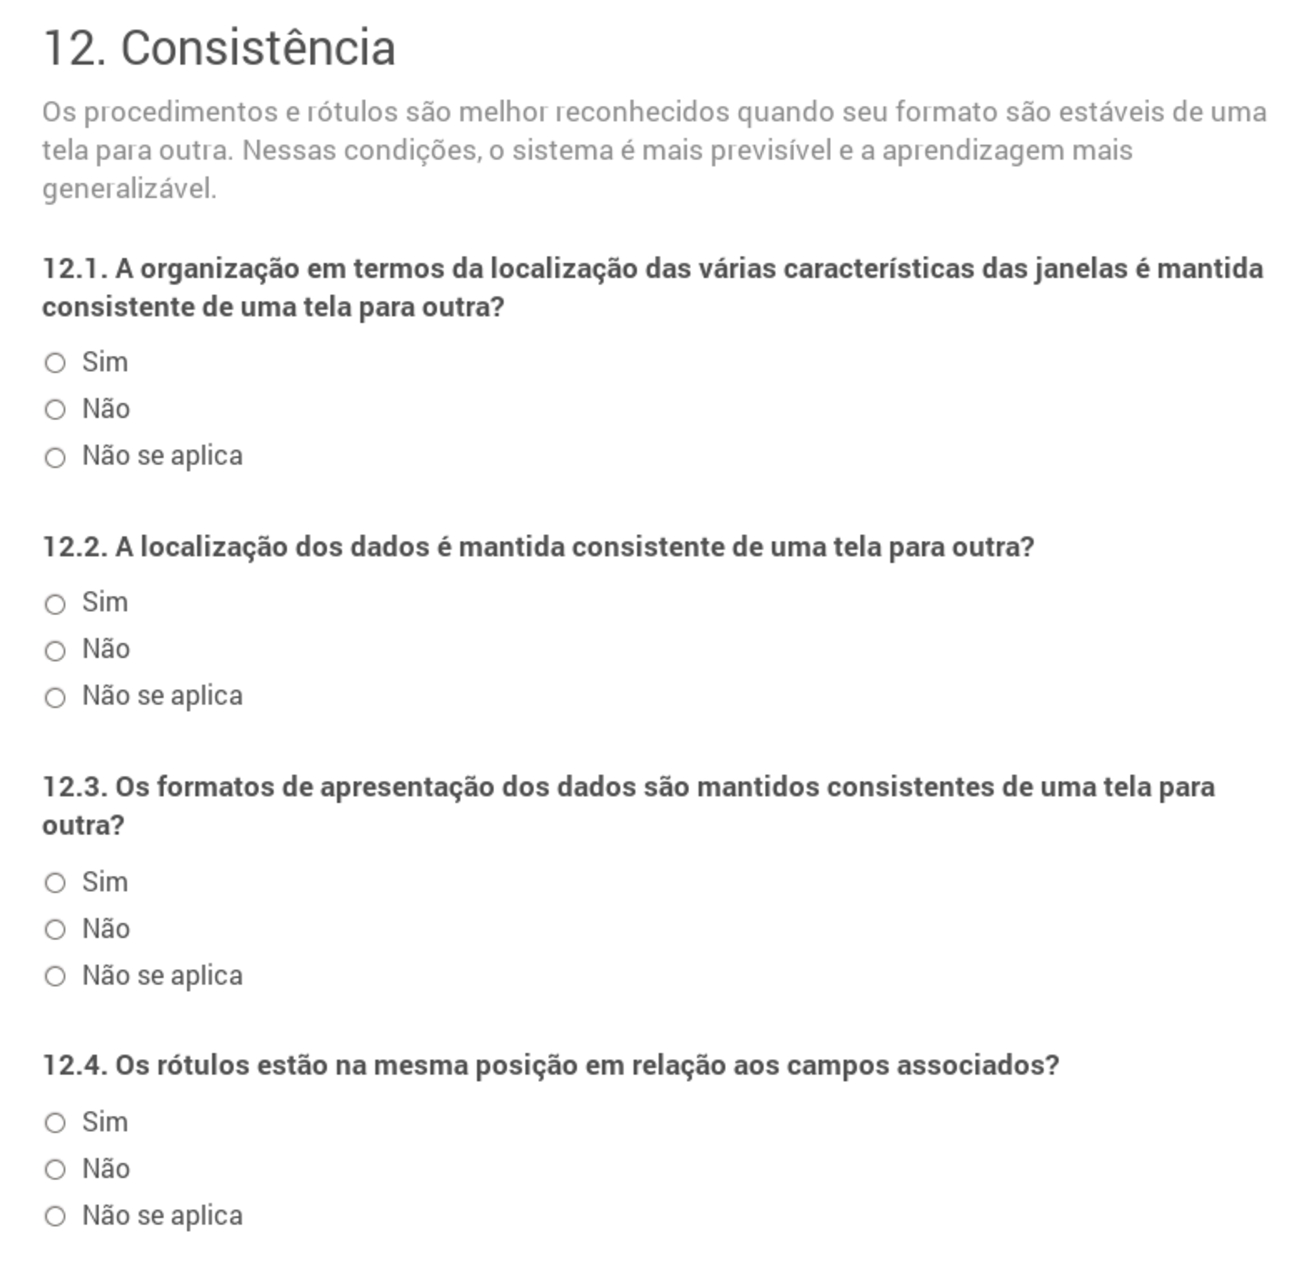
\includegraphics[keepaspectratio=true,scale=0.55]
      		{figuras/check12.eps}
    	\label{check04}
		\caption{Checklist de usabilidade- Questões da seção 12}
	\end{figure}

\newpage